\chapter{Design Objectives}
\label{three}

In this chapter we will discuss about our overall goal for using LLVM as a new Parabix back end. First, we would show that the IDISA library could be replace by a pure target-independent IR library.

To start, let us look at one IDISA vertical operation: {\tt simd<8>::add}. IDISA library implements this function with the compiler intrinsic that directly translates into the assembly code, so different header files have to be maintained for different instruction sets such as Program~\ref{prog:add_8_sse2} and Program~\ref{prog:add_8_neon}. However, with the LLVM IR, we can implement it as Program~\ref{prog:add_8_llvm}; no low level detail is specified here.

\begin{program}
\begin{verbatim}
  template <> bitblock128_t simd<8>::add(bitblock128_t arg1, bitblock128_t arg2)
  {
    return _mm_add_epi8(arg1, arg2);
  }
\end{verbatim}
\caption{Implementation of {\tt simd<8>::add} for X86 SSE2}
\label{prog:add_8_sse2}
\end{program}

\begin{program}
\begin{verbatim}
  template <> bitblock128_t simd<8>::add(bitblock128_t arg1, bitblock128_t arg2)
  {
    return (bitblock128_t)vaddq_u8((uint8x16_t)(arg1), (uint8x16_t)(arg2));
  }
\end{verbatim}
\caption{Implementation of {\tt simd<8>::add} for ARM NEON}
\label{prog:add_8_neon}
\end{program}

\begin{program}
\begin{verbatim}
  define <16 x i8> @simd_add_8(<16 x i8> %arg1, <16 x i8> %arg2) {
  entry:
    %r = add <16 x i8> %arg1, %arg2
    ret <16 x i8> %r
  }
\end{verbatim}
\caption{Implementation of {\tt simd<8>::add} with LLVM IR}
\label{prog:add_8_llvm}
\end{program}

\begin{program}
\begin{verbatim}
  define <16 x i8> @simd_eq_8(<16 x i8> %arg1, <16 x i8> %arg2) {
  entry:
    %r1 = icmp eq <16 x i8> %arg1, %arg2
    %r2 = sext <16 x i1> %r1 to <16 x i8>
    ret <16 x i8> %r2
  }
\end{verbatim}
\caption[Implementation of {\tt simd<8>::eq} with LLVM IR]{Implementation of {\tt simd<8>::eq} with LLVM IR. {\tt Sext} is the instruction for sign extension.}
\label{prog:icmp}
\end{program}

\begin{program}
\begin{verbatim}
  define <16 x i8> @simd_max_8(<16 x i8> %a, <16 x i8> %b) {
  entry:
    %m = icmp sgt <16 x i8> %a, %b
    %r = select <16 x i1> %m, <16 x i8> %a, <16 x i8> %b
    ret <16 x i8> %r
  }
\end{verbatim}
\caption[Implementation of {\tt simd<8>::max} with LLVM IR]{Implementation of {\tt simd<8>::max} with LLVM IR. {\tt Select} would select elements according to the first operand: $\text{\tt r}_i=
\begin{cases}
    \text{\tt a}_i& \text{if } \text{\tt m}_i = 1\\
    \text{\tt b}_i& \text{otherwise}
\end{cases}$.}
\label{prog:max}
\end{program}

Most of the IDISA vertical operations can be expressed with a few lines of IR code. A bit more examples are listed here:

\begin{itemize}
    \item Vector addition, subtraction, multiplication and shifting. There are IR instructions that correspond one-to-one with them.
    \item Integer comparison such as equality, greater than and unsigned less than. In IR, there is one instruction called `icmp' which does the comparison. The only difference is that for vector type {\tt <N x iX>}, the comparison result of `icmp' is in type {\tt <N x i1>} while IDISA requires it to be in type {\tt <N x iX>} (All ones in an element means true and all zeros means false). We need to perform a sign extension by coping the sign bit of the $i1$ result until it reaches the size of $iX$ (Program~\ref{prog:icmp}).
    \item Operations that have no IR correspondence such as {\tt simd::min} and {\tt simd::max}. They can be emulated with a sequence of IR, e.g.\ {\tt simd<8>::max} in Program~\ref{prog:max}.
\end{itemize}

For horizontal operations, IDISA also needs to maintain target-specific logic. For example, to implement {\tt hsimd<16>::packh}, it uses unsigned saturation $packuswb$ for X86 SSE2 and uses $vuzpq\_u8$ for NEON; for X86 SSE series after SSSE3, it would use the instruction $pshufb$. The author of the IDISA library needs to know these instruction sets very well. On the other hand, LLVM IR introduces a powerful instruction which can express most of the horizontal and expansion operations. It is the \textit{shufflevector}.

\begin{verbatim}
    <result> = shufflevector <n x <ty>> <v1>, <n x <ty>> <v2>, <m x i32> <mask>
    ; yields <m x <ty>>
\end{verbatim}

The first two operands are vectors of the same type and their elements are numbered from left to right across the boundary. In the other word, the element indexes are $0$ \ldots $n-1$ for {\tt v1} and $n$ \ldots $2n-1$ for {\tt v2}. The {\tt mask} is an array of constant integer indexes, which indicates the elements we want to extract to form the {\tt result}. Either {\tt v1} or {\tt v2} can be "undefined" to do shuffle within one vector. Shufflevector is often used together with the \textit{bitcast} operation. It converts between integer, vector and FP-values and changes the data type without moving or modifying the data, thus requiring the source and result type to have the same size in bits. With shufflevector and bitcast, we could write {\tt hsimd<32>::packh} in Program~\ref{program:packh_32}. Figure~\ref{figure:packh_32} explains the indexes used in the shuffle mask.

\begin{figure}[ht!]
\centering
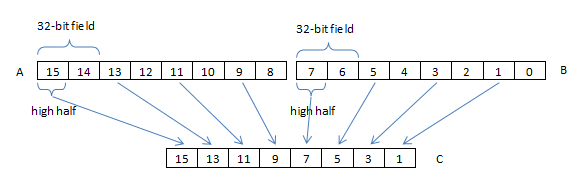
\includegraphics[width=130mm]{draw/packh_16.png}
\caption[Implement {\tt hsimd<32>::packh} with shufflevector]{Shufflevector and {\tt hsimd<32>::packh}. The vectors are bitcasted into $v8i16$ and the indexes for the shuffle mask are drawn in the cell.}
\label{figure:packh_32}
\end{figure}

\begin{program}
\begin{verbatim}
  define <8 x i16> @hsimd_packh_32(<4 x i32> %a, <4 x i32> %b) {
  entry:
    %aa = bitcast <4 x i32> %a to <8 x i16>
    %bb = bitcast <4 x i32> %b to <8 x i16>
    %rr = shufflevector <8 x i16> %bb, <8 x i16> %aa, <8 x i32> <i32 1, i32 3,
          i32 5, i32 7, i32 9, i32 11, i32 13, i32 15>

    ret <8 x i16> %rr
  }
\end{verbatim}
\caption[Shufflevector implementation of packh.]{Shufflevector and {\tt hsimd<32>::packh} in LLVM IR\@. Horizontal operations half the width of fields and that effect is reflected in the return value type.}
\label{program:packh_32}
\end{program}

Program~\ref{program:packh_32} can be easily generalized for packing high on any power-of-two field width. For other horizontal operations:
\begin{itemize}
    \item Packing low: the same bitcast need to be done but shufflevector with a different mask. E.g.\ {\tt hsimd<32>::packl} can be implemented with the mask {\tt 0, 2, 4, 6, 8, 10, 12, 14}.
    \item Packing sign mask: it packs together all the sign bits from each field of the operand and this can be implemented with the less than comparison. E.g.\ {\tt hsimd<32>::signmask(a)} is equivalent to \verb|icmp slt <4 x i32> %a, <4 x i32> <i32 0, i32 0, i32 0, i32 0>| which would return a {\tt <4 x i1>} sign mask vector.
    \item Other operations that require coding a sequence of IR like {\tt hsimd<32>::add\_hl(a, b)}. They are less frequently used in the Parabix application.
\end{itemize}

Shufflevector and bitcast could also cover IDISA expansion operations. We list the IR code for {\tt esimd<16>::mergeh} in Program~\ref{prog:mergeh_16} and explain the indexes in Figure~\ref{fig:mergeh_16}. The program is self-explanatory and any programmer who understands shufflevector can understand its behavior easily.

\begin{program}
\begin{verbatim}
  define <4 x i32> @esimd_mergeh_16(<8 x i16> %a, <8 x i16> %b) {
  entry:
    %rr = shufflevector <8 x i16> %b, <8 x i16> %a, <8 x i32> <i32 4, i32 12,
          i32 5, i32 13, i32 6, i32 14, i32 7, i32 15>

    %rr1 = bitcast <8 x i16> %rr to <4 x i32>
    ret <4 x i32> %rr1
  }
\end{verbatim}
\caption[Shufflevector implementation of mergeh.]{Shufflevector and {\tt esimd<16>::mergeh} in LLVM IR\@. Vertical operations double the width of fields.}
\label{prog:mergeh_16}
\end{program}

The rest expansion operations can be implemented with the same technique. For field movement operations, LLVM IR offers two other vector instructions {\tt insertelement} and {\tt extractelement} to insert or extract fields from the vector; unary movement like rotation of fields within one SIMD register can be implemented with shufflevector. The full register operations could be written in large-size integers like $i128$ and $i256$. All the integer instructions LLVM support can be applied to them thus enabling more complexed operations that IDISA does not support.

To sum up, with support of all the five categories of IDISA operations,
